\chapter{Line-of-Sight Channel - Narrowband Analysis}
\label{chap:los}

The analysis begins with the simplest communication scenario: a direct Line-of-Sight ray between the transmitter TX and the receiver RX. A narrowband analysis is conducted, which assumes that the signal's bandwidth is much smaller than the channel's coherence bandwidth. This simplification allows the channel to be characterized by one complex coefficient.

The physical channel can be described by its time-variant impulse response, which for a set of $N$ multiray components is:
\begin{equation}
	h(\tau,t) = \sum_{n=1}^{N} \alpha_n(t) \delta(\tau - \tau_n)
\end{equation}

where $\alpha_n(t)$ and $\tau_n$ are the complex amplitude and propagation delay of the $n$-th ray, respectively.

\begin{figure}[H]
	\centering
	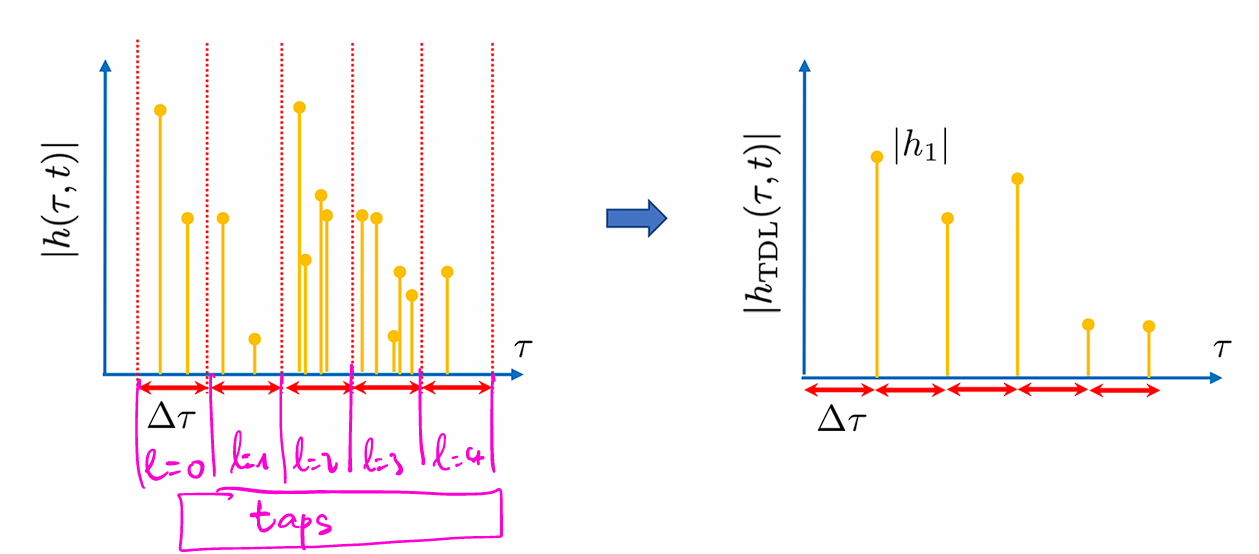
\includegraphics[width=\linewidth]{content/4-images/taps}
	\caption[Physical impulse response and TDL model under the Uncorrelated Scattering assumption]{Physical impulse response and TDL model under the Uncorrelated Scattering assumption\footnotemark}
	\label{fig:taps}
\end{figure}
\footnotetext{The US assumption posits that the complex amplitudes of multipath components arriving at different delays are statistically uncorrelated, meaning they are independent from one another}

A practical communication system has a finite bandwidth $B$, which limits its ability to resolve rays arriving at different times. The system's time resolution is $\Delta\tau = 1/B$. 

The received signal is defined by:
\begin{equation}
	y(t) = \sum_l x(t-l \Delta \tau) \underbrace{\int_0^{\infty} h(\tau, t) \operatorname{sinc}(B(\tau-l \Delta \tau)) d \tau}_{h_l(t)}
\end{equation}

From there, can be defined the complex gain of the $l$-th tap:
\begin{align}
	h_l(t) &= \int_0^{\infty} h(\tau, t) \operatorname{sinc}(B(\tau-l \Delta \tau)) d \tau \\
	&= \int_0^{\infty} (\sum_{n=1}^{N} \alpha_n(t) \delta(\tau - \tau_n)) \cdot \operatorname{sinc}(B(\tau-l \Delta \tau)) d \tau \\
	 &= \sum_{n=1}^N \alpha_n(t) \operatorname{sinc}\left(B\left(\tau_n-l \Delta \tau\right)\right)
\end{align}

\begin{equation}
	\label{eq:h-l}
	\implies \boxed{h_l(t) \approx \sum_{\tau_n \in \operatorname{tap} l} \alpha_n(t)} 
\end{equation}
Equation \eqref{eq:h-l} can be written because $\operatorname{sinc(.)}$ maximizes the amplitude of the components of the  $l$-th tap, and the components of other taps are drastically attenuated. The components of the $l$-th tap appear not to be delayed between one another.

The physical limitation of the finite bandwidth of the system leads to the Tapped Delay Line model. The impulse response of the TDL model is a discrete-time representation of the physical channel as shown in Figure \ref{fig:taps}:
\begin{equation}
	h_{TDL}(\tau, t) = \sum_{l=0}^{L} h_l(t) \delta(\tau - l\Delta\tau)
	\label{eq:tdl_model}
\end{equation}


The condition for a narrowband channel is that the signal bandwidth $B$ is much smaller than the channel's coherence bandwidth $\Delta f_c$. The coherence bandwidth is inversely proportional to the channel's delay spread, $\sigma_\tau = max|\tau_i - \tau_j|$. The narrowband condition is thus expressed as:
\begin{equation}
	B \ll \Delta f_c \approx \frac{1}{\sigma_\tau} \implies \Delta\tau \gg \sigma_\tau
\end{equation}

This inequality means the system's time resolution is much larger than the delay spread. From the receiver's perspective, all MPCs arrive at effectively the same time. Consequently, all MPCs fall into the first tap ($l=0$) of the TDL model. The summation in Equation \eqref{eq:tdl_model} therefore reduces to one term for $l=0$:
\begin{equation}
	\label{eq:tdl-narrow}
	h_{TDL}(\tau, t) = h_0(t) \delta(\tau)
\end{equation}

where the tap gain $h_0(t)$ is the sum of all individual ray gains:
\begin{equation}
	\label{eq:narrow}
	\boxed{h_0(t) = \sum_{n=1}^{N} \alpha_n(t)} \quad N \text{ being the total number of MPCs}
\end{equation}


\section{Antenna Gain}
The gain of an antenna, $G(\theta, \phi)$, quantifies its ability to concentrate radiated power in a specific direction. It is defined by the general formula:
\begin{equation}
	G(\theta,\phi) = \frac{\pi Z_0}{R_a} \frac{|\vec{h}_{e\perp}(\theta,\phi)|^2}{\lambda^2}
	\label{eq:gain_general}
\end{equation}
where $Z_0$ is the impedance of free space, $R_a$ is the antenna's radiation resistance, $\lambda$ is the wavelength, and $\vec{h}_{e\perp}(\theta,\phi)$ is the transverse component of the antenna's effective height.

As derived earlier (Equation \ref{eq:he_perp_horizontal}), the transverse effective height for a vertical half-wave dipole in the horizontal plane ($\theta = \frac{\pi}{2}$) is:
\begin{equation}
	\vec{h}_{e\perp}\left(\frac{\pi}{2},\phi\right) = -\frac{\lambda}{\pi}\vec{1}_{\theta}
\end{equation}

The magnitude squared of this vector is therefore:
\begin{equation}
	\left|\vec{h}_{e\perp}\left(\frac{\pi}{2},\phi\right)\right|^2 = \left|-\frac{\lambda}{\pi}\vec{1}_{\theta}\right|^2 = \frac{\lambda^2}{\pi^2}
\end{equation}

Substituting this result into the general gain Equation \eqref{eq:gain_general} provides the expression for the gain of a lossless half-wave dipole in the horizontal plane:
\begin{equation}
	G = G\left(\frac{\pi}{2}, \phi\right) = \frac{\pi Z_0}{R_a} \frac{1}{\lambda^2} \left(\frac{\lambda^2}{\pi^2}\right) = \frac{\pi Z_0 \lambda^2}{\pi^2 R_a \lambda^2}
\end{equation}
Simplifying this expression yields the final result:
\begin{equation}
	G = \frac{Z_0}{\pi R_a}
	\label{eq:gain_derived}
\end{equation}

\section{Impulse Response $h(\tau)$}
For a single, time-invariant Line-of-Sight ray, the channel impulse response is characterized by a single complex amplitude, $\alpha_1$, and a propagation delay, $\tau_1$. The impulse response is thus expressed as:
\begin{equation}
	h(\tau) = \alpha_1 \delta(\tau - \tau_1)
\end{equation}
The complex amplitude $\alpha_1$ has to be determined. This can be achieved by relating the circuit-level voltages at the transmitter and receiver. The relationship between the transmitted power $P_{TX}$ and the received power $P_{RX}$ is defined by the squared magnitude of the complex amplitude:
\begin{equation}
	P_{RX} = |\alpha_1|^2 P_{TX}
\end{equation}
The transmitted and received powers can be expressed in terms of the terminal voltages $\underline{V}_{TX}$ and $\underline{V}_{RX}$ and the antenna radiation resistance $R_a$, assuming perfectly matched conditions:
\begin{equation}
	P_{TX} = \frac{1}{2} R_a |\underline{I}_a|^2 = \frac{1}{2} R_a \frac{|\underline{V}_{TX}|^2}{4R_a^2} = \frac{|\underline{V}_{TX}|^2}{8R_a} 
\end{equation}
\begin{equation}
	P_{RX} = \frac{1}{2} R_a |\underline{I}_a|^2 = \frac{1}{2} R_a \frac{|\underline{V}_{RX}|^2}{R_a^2}= \frac{|\underline{V}_{RX}|^2}{2R_a}
\end{equation}
Substituting these power definitions into the power relationship gives:
\begin{equation}
	\frac{|\underline{V}_{RX}|^2}{2R_a} = |\alpha_1|^2 \frac{|\underline{V}_{TX}|^2}{8R_a}
\end{equation}
Solving for $|\alpha_1|^2$ yields:
\begin{equation}
	|\alpha_1|^2 = \frac{8R_a}{2R_a} \frac{|\underline{V}_{RX}|^2}{|\underline{V}_{TX}|^2} = 4 \frac{|\underline{V}_{RX}|^2}{|\underline{V}_{TX}|^2}
\end{equation}
This implies a relationship between the magnitudes: $|\alpha_1| = 2 \frac{|\underline{V}_{RX}|}{|\underline{V}_{TX}|}$. This motivates defining the complex amplitude $\alpha_1$ directly from the complex voltage ratio:
\begin{equation}
	\alpha_1 = 2 \frac{\underline{V}_{RX}}{\underline{V}_{TX}}
	\label{eq:alpha_from_voltages}
\end{equation}
The relationship between the received and transmitted voltages for a free-space LOS ray was derived previously in Equation \eqref{eq:VRX_vs_VTX} as:
\begin{equation}
	\underline{V}_{RX} = j \frac{\lambda Z_0}{8\pi^2 R_a c\tau_1} \underline{V}_{TX} e^{-j2\pi f_c \tau_1}
\end{equation}
Substituting this into Equation \eqref{eq:alpha_from_voltages} gives the expression for $\alpha_1$:
\begin{equation}
	\alpha_1 = 2 \left( j \frac{\lambda Z_0}{8\pi^2 R_a c\tau_1} e^{-j2\pi f_c \tau_1} \right) = j \frac{\lambda Z_0}{4\pi^2 R_a c\tau_1} e^{-j2\pi f_c \tau_1}
\end{equation}
Replacing the product of the speed of light $c$ and the delay $\tau_1$ with the distance $d_1 = c\tau_1$, the complex amplitude is:
\begin{equation}
	\alpha_1 = j \frac{\lambda Z_0}{4\pi^2 R_a d_1} e^{-j2\pi f_c \tau_1}
	\label{eq:alpha1_derived}
\end{equation}
The channel impulse response for the LOS ray is therefore:
\begin{equation}
	\boxed{h(\tau) = \left( j \frac{\lambda Z_0}{4\pi^2 R_a d_1} e^{-j2\pi f_c \tau_1} \right) \delta(\tau - \tau_1)}
	\label{eq:los_impulse_response_derived_detailed}
\end{equation}
where $\tau_1 = d_1/c$.

\section{Transfer Function $H(f)$}
The transfer function $H(f)$ is obtained by taking the Fourier transform of the impulse response $h(\tau)$:
\begin{equation}
	H(f) = \mathcal{FT}\{ h(\tau)\} =  \int_{-\infty}^{\infty} h(\tau) e^{-j2\pi f \tau} d\tau = \int_{-\infty}^{\infty} \left( \alpha_1 \delta(\tau - \tau_1) \right) e^{-j2\pi f \tau} d\tau
\end{equation}
Applying the sifting property of the Dirac delta function, which states that $\int g(x)\delta(x-a)dx = g(a)$, the integral simplifies to:
\begin{equation}
	H(f) = \alpha_1 e^{-j2\pi f \tau_1}
\end{equation}
Substituting the derived expression for $\alpha_1$ from Equation \eqref{eq:alpha1_derived}:
\begin{align}
	H(f) &= \left( j \frac{\lambda Z_0}{4\pi^2 R_a d_1} e^{-j2\pi f_c \tau_1} \right) e^{-j2\pi f \tau_1} \\
	\Rightarrow \Aboxed{H(f) &= j \frac{\lambda Z_0}{4\pi^2 R_a d_1} e^{-j2\pi (f_c + f) \tau_1}}
	\label{eq:los_transfer_function_detailed}
\end{align}
This function shows that the channel introduces a phase shift that is linear with the baseband frequency $f$, which corresponds to the time delay $\tau_1$. The magnitude $|H(f)|$ is constant across all frequencies.

\section{Narrowband Transfer Function $h_{NB}$}
As said in Equation \eqref{eq:tdl-narrow}, the narrowband is defined such that all MPCs fall into a single tap:
\begin{align}
	h_{NB} &= \mathcal{FT}\{ h_{TDL}(t, \tau)\} = \mathcal{FT}\{ h_{0}(t)\delta(\tau)\} \\
	&= \int_{-\infty}^{\infty} h_0(t) e^{-j2\pi f \tau} \delta(\tau) d\tau \\
	&=h_0(t)e^{-j2\pi f \cdot \hspace{0.05em} 0} \\
	\implies \Aboxed{h_{NB} &= h_0(t)}
\end{align}

As found in Equation \eqref{eq:narrow}, for a single LOS ray, the narrowband channel transfer function is equal to the complex amplitude $\alpha_1$:
\begin{equation}
	h_{NB} = \sum_{n=1}^{N=1} \alpha_n(t) = \alpha_1
\end{equation}
Using the result from Equation \eqref{eq:alpha1_derived}, the narrowband transfer function is:
\begin{equation}
	\boxed{h_{NB} = j \frac{\lambda Z_0}{4\pi^2 R_a d_1} e^{-j2\pi f_c \tau_1}}
	\label{eq:los_narrowband_tf_detailed}
\end{equation}
The LOS channel is thus represented by one complex number, which scales and rotates the transmitted signal.

\section{Received Power $P_{RX}$}
The received power can now be calculated using the derived complex amplitude $\alpha_1$ and its relationship to the power gain, $P_{RX} = |\alpha_1|^2 P_{TX}$. First, the magnitude squared of $\alpha_1$ is computed:
\begin{equation}
	|\alpha_1|^2 = \left| j \frac{\lambda Z_0}{4\pi^2 R_a d_1} e^{-j2\pi f_c \tau_1} \right|^2 = \left( \frac{\lambda Z_0}{4\pi^2 R_a d_1} \right)^2
\end{equation}
Substituting this into the power equation gives the received power as a function of the transmitted power:
\begin{equation}
	\boxed{P_{RX} = \left( \frac{\lambda Z_0}{4\pi^2 R_a d_1} \right)^2 P_{TX}}
\end{equation}
To demonstrate that this result is equivalent to the Friis formula, the terms are rearranged. The expression is factored to isolate terms corresponding to the antenna gains:
\begin{align}
	P_{RX} &= \frac{\lambda^2 Z_0^2}{16\pi^4 R_a^2 d_1^2} P_{TX} \\
	&= \left( \frac{Z_0^2}{\pi^2 R_a^2} \right) \left( \frac{\lambda^2}{16\pi^2 d_1^2} \right) P_{TX} \\
	&= \left( \frac{Z_0}{\pi R_a} \right) \left( \frac{Z_0}{\pi R_a} \right) \left( \frac{\lambda}{4\pi d_1} \right)^2 P_{TX}
\end{align}
Using the expression for the gain of a lossless half-wave dipole in the horizontal plane as derived in Equation \eqref{eq:gain_derived}, $G = Z_0/(\pi R_a)$, and assuming identical transmit and receive antennas ($G_{TX} = G_{RX} = G$):
\begin{equation}
	P_{RX} = G_{TX} G_{RX} \left( \frac{\lambda}{4\pi d_1} \right)^2 P_{TX} \label{eq:los_power_final_detailed}
\end{equation}
This result is identical to the Friis transmission formula. This validates the entire derivation, confirming that the complex amplitude $\alpha_1$ derived from the voltage ratio correctly predicts the power relationship under free-space LOS conditions.

\section{Interpretation of Results}
The derivations confirm the principles of a simple LOS communication link.
\begin{itemize}
	\item \textbf{Frequency-Flat Channel:} The single propagation ray results in a transfer function $|H(f)|$ that is constant with frequency. This means the channel does not distort the signal's spectrum, illustrating flat fading. This is a direct consequence of having no time dispersion, meaning zero delay spread).
	\item \textbf{Validation of Friis' Formula:} The derivation, starting from the circuit-level voltage relationship to find the complex amplitude $\alpha_1$, and then using it to find the received power, shows a result identical to the Friis' formula.
\end{itemize}
